\documentclass[a4paper]{article}
\usepackage{a4wide}
\usepackage{makeidx}
\usepackage{fancyhdr}
\usepackage{graphicx}
\usepackage{multicol}
\usepackage{float}
\usepackage{textcomp}
\usepackage{alltt}
\usepackage{times}
\usepackage{ifpdf}
\ifpdf
\usepackage[pdftex,
            pagebackref=true,
            colorlinks=true,
            linkcolor=blue,
            unicode
           ]{hyperref}
\else
\usepackage[ps2pdf,
            pagebackref=true,
            colorlinks=true,
            linkcolor=blue,
            unicode
           ]{hyperref}
\usepackage{pspicture}
\fi
\usepackage[utf8]{inputenc}
\usepackage{doxygen}
\makeindex
\setcounter{tocdepth}{3}
\newcommand{\Hrule}[1]{\rule{\linewidth}{#1}}
\newcommand{\codeversion}{1.1}
\newcommand{\doctitle}{Reference Manual}
\newcommand{\avmesh}{\emph{AVMesh Format \& Library}}
\usepackage{colortbl}
\definecolor{lightGray}{gray}{0.75}
\renewcommand{\footrulewidth}{0.4pt}
\begin{document}
\pagenumbering{arabic}
\begin{titlepage}
  \thispagestyle{empty}

  \begin{flushright}

    \colorbox{lightGray}
      {\begin{minipage}[c]{2.0in}
        \begin{center}
          \vspace{6pt}
          \textbf{\Large{Version}} \\
          \vspace{8pt}
          \textcolor{white}{\fontsize{90}{100}\bfseries \codeversion}
          \vspace{6pt}
        \end{center}  
      \end{minipage}}

  \end{flushright}

  \vspace{0.25in}

  \begin{flushleft}
    
    \huge { Computational Research and Engineering 
    Acquisition Tools And Environments (CREATE) }
    \Hrule{1.0pt} \\
    \Huge Air Vehicles

  \end{flushleft}

  \vspace{0.75in}
  
  \begin{centering}

    
\includegraphics[height=0.085\textheight]{createLogo.pdf} 
    \hfill
    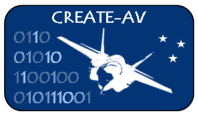
\includegraphics[height=0.085\textheight]{createAVLogo.pdf}

  \end{centering}

  \vspace{0.75in}

  \begin{center}

    \colorbox{lightGray}
      {\begin{minipage}[c]{0.98\textwidth}
        \begin{flushright}
          \vspace{16pt}
          
          {\fontsize{36}{72}\normalfont \avmesh} \\
          \vspace{16pt}
          {\fontsize{40}{72}\normalfont \doctitle}  
          
          \vspace{16pt}
        \end{flushright}
      \end{minipage}}

    \vspace{0.5in}

  \end{center}

\end{titlepage}


\tableofcontents
\newpage
\part{Overview}
\section{Introduction}
\label{index}\hypertarget{index}{}\input{index}
\newpage
\section{Library Installation Guide}
\label{install_guide}
\hypertarget{install_guide}{}
\input{install_guide}
\newpage
\section{Library Usage Guide}
\label{quick_example}
\hypertarget{quick_example}{}
\input{quick_example}
\newpage
\part{Format Reference}
\section{AVMesh Rev1 File and Generic Mesh Header Format}
\label{avmhdrs}
\hypertarget{avmhdrs_rev1}{}
\input{avmhdrs_rev1}
\newpage
\section{Unstructured Data Format}
\label{unstruc}
\hypertarget{unstruc_rev1}{}
\input{unstruc_rev1}
\newpage
\section{Strand Data Format}
\label{strand}
\hypertarget{strand_rev1}{}
\input{strand_rev1}
\newpage
\section{Body-Fitted Structured Data Format}
\label{bfstruc}
\hypertarget{bfstruc_rev1}{}
\input{bfstruc_rev1}
\newpage
\section{Cartesian Data Format}
\label{cart}
\hypertarget{cart_rev1}{}
\input{cart_rev1}
\newpage
\part{Library Reference}
\section{API Reference}
\input{group__api}
\section{Type Reference}
\input{structfile__id__prefix__t}
\input{structrev1_1_1file__header__t}
\input{structrev1_1_1mesh__header__t}
\input{structrev1_1_1bfstruc__header__t}
\input{structrev1_1_1bfstruc__patch__t}
\input{structrev1_1_1cart__header__t}
\input{structrev1_1_1cart__block__t}
\input{structrev1_1_1strand__header__t}
\input{structrev1_1_1strand__edge__patch__t}
\input{structrev1_1_1strand__surf__patch__t}
\input{structrev1_1_1unstruc__header__t}
\input{structrev1_1_1unstruc__patchheader__t}
\printindex
\end{document}
